\section{Cross talk measutrements}

Electronic crosstalk is present in both the H12700 and H8500 MAPMTs. To demonstrate this, we collected data where all pixels on a single MAPMT were masked with a sheet of black paper, and a 3mm diameter hole was punctured over a single pixel. Despite the laser light only being incident on the single unmasked pixel, we observed signals in the surrounding pixels whose amplitudes were in fact proportional to the amplitude of the corresponding signal in the unmasked pixel. Fig.~\ref{fig:H12700pinhole} and Fig.~\ref{fig:H8500pinhole} show the measured charge spectra for a cluster of pixels in an H12700 MAPMT and an H8500 MAPMT (respectively) when only the central pixel (in this case, pixel 28) was unmasked. The signals above pedestal in the surrounding pixels predominantly originate from crosstalk of the electron cascade in the dynodes of pixel 28. 

\begin{figure*}
	\centering
	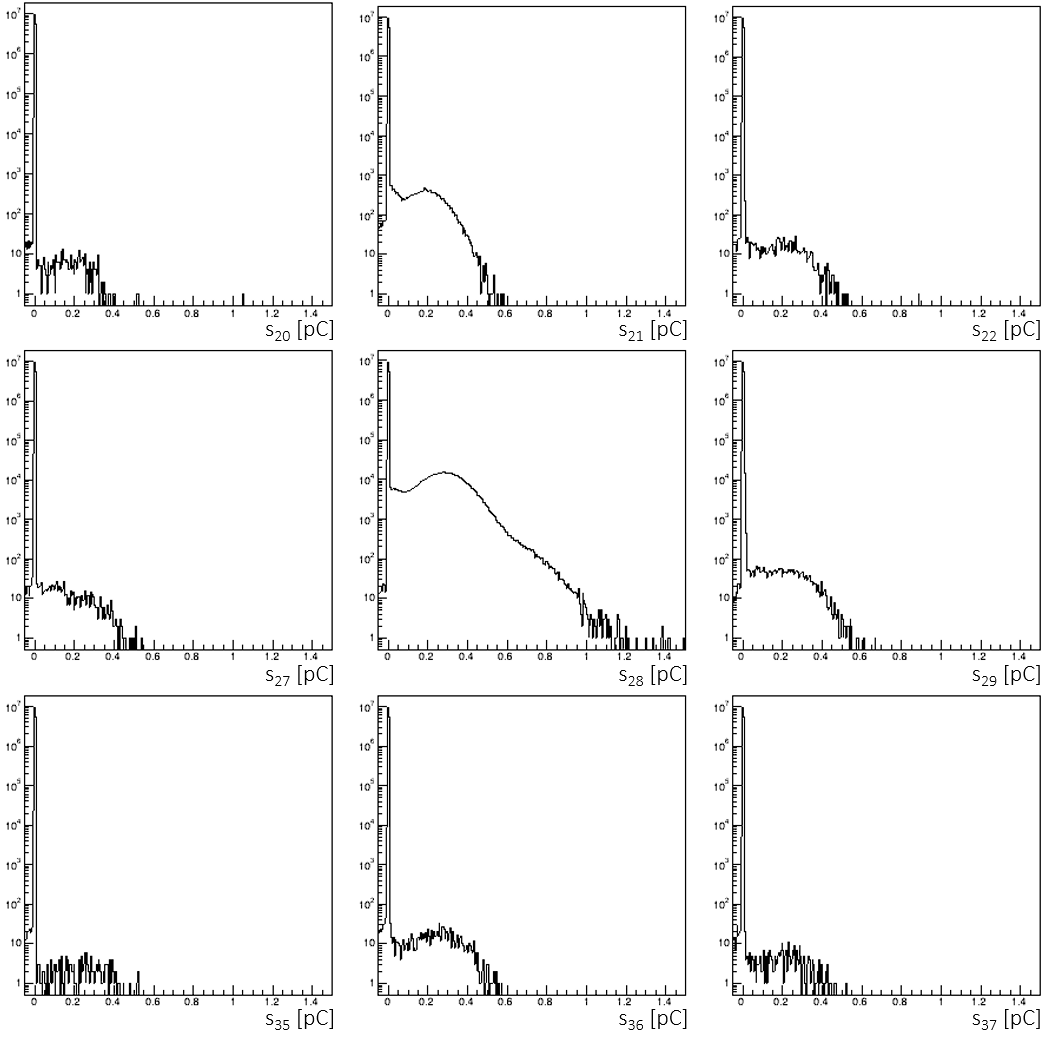
\includegraphics[width=0.95\linewidth]{figures/H12700_pixel28_pinhole.png}
	\caption{The charge spectra for pixel 28 of a typical H12700 MAPMT and the surrounding pixels when only pixel 28 was illuminated by the laser light.}
	\label{fig:H12700pinhole}
\end{figure*}
\begin{figure*}
	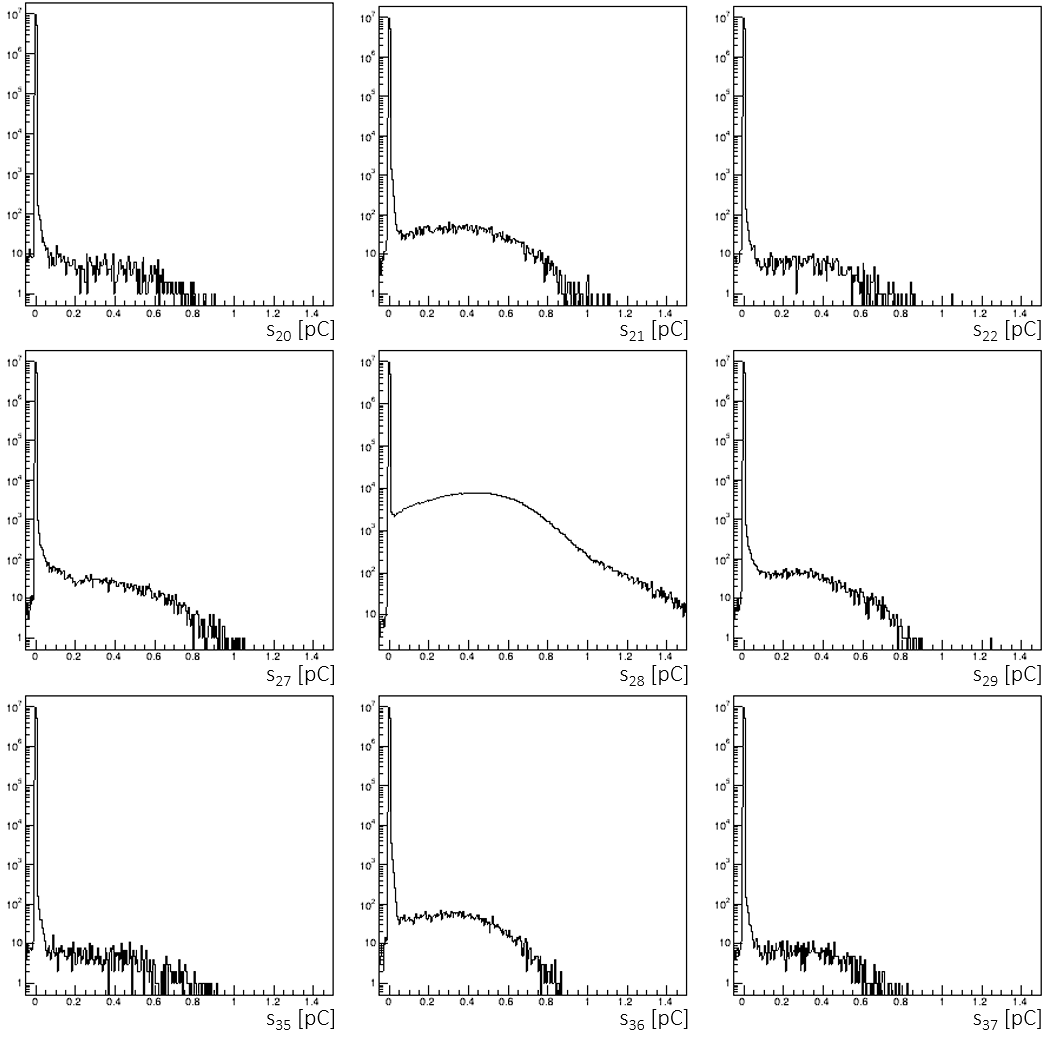
\includegraphics[width=0.95\linewidth]{figures/H8500_pixel28_pinhole.png}
	\caption{The charge spectra for pixel 28 of a typical H8500 MAPMT and the surrounding pixels when only pixel 28 was illuminated by the laser light.}
	\label{fig:H8500pinhole}
\end{figure*}

The crosstalk changes the shape of the measured charge spectra by adding a "shoulder" to the right side of the pedestal region. Thus, to properly characterize the single photoelectron spectrum for each pixel, one needs to either add a description of the crosstalk into the mathematical model for the s.p.e. response, or one can attempt to identify and remove these crosstalk events from the data. A simple procedure was developed and implemented to attempt the latter option. Because the amplitude of the crosstalk is linearly dependent on the amplitude of the photo-induced signal, the crosstalk events appear as linear bands in the plots showing the measured charge in one pixel as a function of the measured charge in a neighboring pixel. Fig.~\ref{fig:H12700neighbors} and Fig.~\ref{fig:H8500neighbors} show these two dimensional plots for all pixels which neighbor pixel 28 for one H12700 MAPMT and one H8500 MAPMT, respectively. From these two plots it is obvious that the strength of the crosstalk is vastly different between the H12700 and H8500 MaPMTs. On average, the amplitude of the crosstalk in an H12700 MAPMT is only about 2-3$\%$ of the main signal, whereas the crosstalk amplitude in an H8500 MAPMT can be as large as 50$\%$ of the main signal. As we will discuss later, this fact makes it more difficult to address the crosstalk for the H8500 MAPMTs in the mathematical description of the spe response function.

Other noteworthy features from Fig.~\ref{fig:H12700neighbors} and Fig.~\ref{fig:H8500neighbors} are that the crosstalk signals are strongest in the pixels immediately to the right and left of the pixel where light was incident. The crosstalk bands in those pixels have the largest slope. Most of the crosstalk is contained within the 4 pixels which share an edge with the illuminated pixel, as the plots for the pixels on the corners show little correlation with the charge measured in the central pixel.

\begin{figure*}
	\centering
	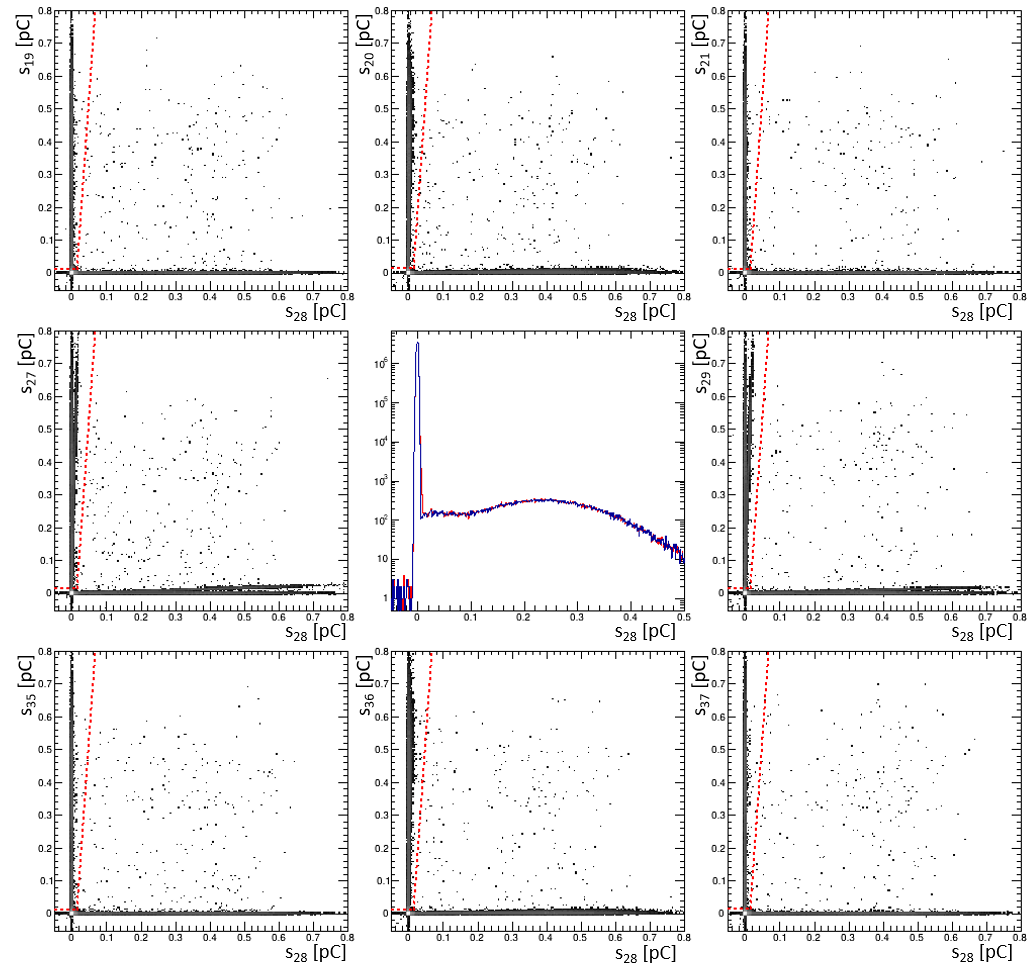
\includegraphics[width=0.95\linewidth]{figures/H12700_ct.png}
	\caption{The charge measured in adjacent pixels is plotted as a function of the charge measured in pixel 28 for a typical H12700 MaPMT. The central plot shows the charge spectrum before (red) and after (blue) removal of the crosstalk events which are cut by the dashed (red) line on the 2-dimenional plots.}
	\label{fig:H12700neighbors}
\end{figure*}
\begin{figure*}
	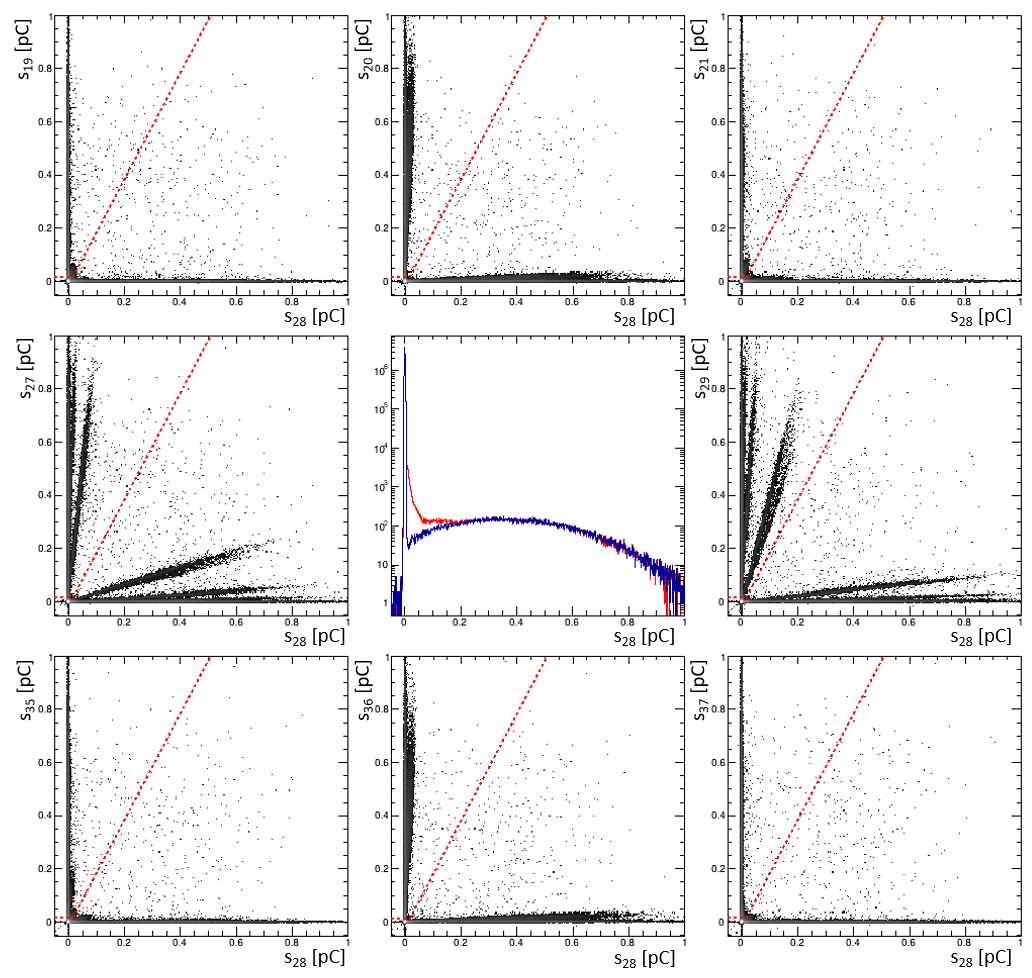
\includegraphics[width=0.95\linewidth]{figures/H8500_ct.png}
	\caption{The charge measured in adjacent pixels is plotted as a function of the charge measured in pixel 28 for a typical H8500 MaPMT. The central plot shows the charge spectrum before (red) and after (blue) removal of the crosstalk events which are cut by the dashed (red) line on the 2-dimenional plots.}
	\label{fig:H8500neighbors}
\end{figure*}

Because the crosstalk events are easily distinguished in these two dimensional plots, a cut can be placed to remove these events from the data. The cut is applied to each pixel separately, and is a linear function of the charge measured in that pixel. Specifically, the cut places a limit on the maximum charge measured in the neighboring pixels. If the maximum neighboring charge is above the cut value for the central pixel$\textquotesingle$s measured charge, then the event is tagged as crosstalk and is removed from the charge spectrum for the central pixel. This cut is shown as a dashed (red) line in Fig.~\ref{fig:H12700neighbors} and Fig.~\ref{fig:H8500neighbors}. The start of the cut line is placed 7$\sigma$ above the pedestal to avoid removing pedestal events. Although the slope of the crosstalk bands can vary between pixels, the slope of the cut line used here is the same for each pixel on a given PMT. 

The main drawback of this crosstalk cut is that it removes events where adjacent pixels both happen to have a photoelectron emitted from the same laser trigger. However, the fraction of these accidental coincidence events is low when the laser filter is used at the minimal setting, meaning at low light intensity this procedure can be used to provide the spe spectrum free from crosstalk. The charge spectra before and after the removal of the crosstalk events in this manner is compared in the central plot in Figs.~\ref{fig:H12700neighbors} and~\ref{fig:H8500neighbors}. For both the H12700 pmt and the H8500 the crosstalk shoulder to the right of the pedestal is removed after applying this cut. 
